\documentclass[conference]{IEEEtran}
\IEEEoverridecommandlockouts
\usepackage{url}
\usepackage{cite}
\usepackage{amsmath,amssymb,amsfonts}
\usepackage{algorithmic}
\usepackage{graphicx}
\usepackage{textcomp}
\usepackage{xcolor}
\usepackage{booktabs}
\usepackage{hyperref}
\def\BibTeX{{\rm B\kern-.05em{\sc i\kern-.025em b}\kern-.08em
    T\kern-.1667em\lower.7ex\hbox{E}\kern-.125emX}}

\begin{document}

\title{Augmenting Mamba-2 with Explicit Memory Caching for Long-Context Recall\\
{\footnotesize CSCI 567 - Machine Learning Final Report}
}

\author{
    \IEEEauthorblockN{Jinglu Sun, Mo Jiang, Zhenglong Liu, and Zhiyuan Jin}
    \IEEEauthorblockA{\textit{University of Southern California} \\
    \{jinglusu, mojiang, zhenglon, jinzhiyu\}@usc.edu}
}

\maketitle

\begin{abstract}
State Space Models (SSMs) such as Mamba-2 offer linear-time sequence modeling but compress all history into a fixed-size recurrent state, which limits exact recall of distant tokens. We augment the pretrained Mamba-2 (1.3B) with two explicit Memory Caching (MC) mechanisms: a sliding-window segment cache (\textbf{Mamba2MC}) and a selective variant that retains only high-scoring segments (\textbf{Mamba2MCSelect}). New parameters are trained on a $\sim$27M-token mix of WikiText and FineWeb using a staged freeze-then-finetune protocol (1 freeze + 2 finetune epochs). We evaluate on WikiText perplexity, three zero-shot reasoning benchmarks (PIQA, HellaSwag, ARC), and a long-context retrieval task (Needle-In-A-Haystack, NIAH). Both MC variants reduce perplexity relative to the pretrained baseline ($10.31 \!\to\! {\approx}\,10.09$), and Mamba2MCSelect outperforms the sliding-window variant on NIAH ($0.90$ vs.\ $0.85$), validating the core selection idea, although neither matches the base Mamba-2's perfect NIAH score ($1.00$). Neither model surpasses the base Mamba-2 on zero-shot reasoning either, a gap we attribute primarily to insufficient fine-tuning data and a short training context length that prevents the selector from being exercised. Code: \url{https://github.com/Ruuuuuush2027/mamba2-optimization}.
\end{abstract}

\begin{IEEEkeywords}
State Space Models, Mamba-2, Memory Caching, Long-Context Recall, Selective Attention, Fine-tuning
\end{IEEEkeywords}

%=============================================================
\section{Introduction}
%=============================================================

Transformer-based models use KV attention to retrieve previous tokens for accurate language understanding. While Transformers are strong at retrieving distant context, this comes at the cost of $O(T)$ memory and $O(T^2)$ compute, where $T$ is the sequence length~\cite{dao2024transformersssmsgeneralizedmodels}. State-space models (SSMs) such as Mamba-2 instead compress historical information into a fixed-size recurrent state, scaling linearly with $T$. However, this compression risks causing the model to ``forget'' specific tokens as it processes new inputs.

To bridge the gap between efficient recursion and accurate recall, we propose appending an explicit, learnable memory buffer to a pre-trained SSM. This approach avoids retraining from scratch and retains the SSM's efficient recursive properties, bridging effective memory use with efficient computation. Our \textbf{core research question} is: can a simple segment-level memory cache, trained solely as new parameters on top of a frozen-then-finetuned SSM backbone, improve long-context recall while preserving the model's general language modelling quality?

\textbf{Related work.}
Hybrid architectures such as Griffin~\cite{de2024griffinmixinggatedlinear} and Jamba~\cite{lieber2024jambahybridtransformermambalanguage} interleave SSM layers with a small number of attention layers---a pragmatic hybrid that sacrifices SSM's linear complexity for a fraction of Transformer's recall ability. Retrieval-augmented LMs~\cite{lewis2021retrievalaugmentedgenerationknowledgeintensivenlp} augment LLMs with an external document store; we borrow the idea of retrieving from a learned memory but operate over the model's own segment-level hidden states rather than a discrete document database, making the entire pipeline end-to-end trainable. The closest prior work is the Compressive Transformer~\cite{rae2019compressivetransformerslongrangesequence}, which maintains a compressed ``memory'' of older activations alongside a standard attention cache; we apply the segment-mean compression idea to an SSM rather than to a Transformer.

%=============================================================
\section{Background: Mamba-2 and the SSD Framework}
%=============================================================

Mamba-2~\cite{dao2024transformersssmsgeneralizedmodels} replaces the standard attention layer with a Structured State Space Dual (SSD) layer. The core recurrence is $h_t = A_t h_{t-1} + B_t x_t,\ y_t = C_t^\top h_t$, where $A_t$ is constrained to scalar-times-identity structure. This yields both an efficient linear recurrent form and a quadratic dual form analogous to masked kernel attention:
\begin{equation}
    Y = (L \circ CB^\top) X,\qquad
    L_{ji} = \begin{cases}\prod_{k=i+1}^{j} a_k & j \ge i \\ 0 & j < i\end{cases}
\end{equation}
The SSD algorithm computes this with a block decomposition that is $2$--$8\times$ faster than Mamba-1's fused scan at the same state size.

Because $h_t$ is a fixed-size vector, the SSM continuously overwrites old information. Empirically, the MQAR associative-recall benchmark~\cite{arora2023zoologymeasuringimprovingrecall}, used in the Mamba-2 evaluation~\cite{dao2024transformersssmsgeneralizedmodels}, shows that SSMs struggle to retrieve exact key--value pairs embedded far in the past. Transformer KV-caches do not have this problem because they store every past key and value explicitly.

%=============================================================
\section{Methods}
%=============================================================

We propose two architectures that add a segment-level memory cache to the pretrained Mamba-2 backbone. Both share the same backbone and differ only in how segments are retained.

\subsection{Mamba2MC: Sliding-Window Segment Cache}

After every $S$ tokens (the \emph{segment size}), we compute a segment hidden state as the mean of the backbone's output hidden states within that window: $\bar{h}_k = \frac{1}{S}\sum_{t=kS}^{(k+1)S-1} h_t$. Up to $K_{\max}$ such segments are retained in a buffer (oldest evicted first). At inference step $t$, before producing the logit for the current token, we blend the SSM's hidden state $h_t$ with a weighted sum over the segment buffer:
\begin{align}
    q &= h_t W,\quad W \in \mathbb{R}^{d \times d} \label{eq:query} \\
    \alpha_k &= \mathrm{softmax}_k\!\left(\frac{q \cdot \bar{h}_k}{\sqrt{d}}\right) \label{eq:scores} \\
    \tilde{h}_t &= \sigma(\beta)\, h_t + (1 - \sigma(\beta))\sum_{k} \alpha_k\, \bar{h}_k \label{eq:mix}
\end{align}
where $W$ is a trainable projection (initialised to the identity), $\beta$ is a trainable scalar gate (initialised to $8.0$ so $\sigma(\beta)\!\approx\!1$, i.e.\ identity behaviour at the start of training), and the softmax is taken over the segment index $k$. The logit is computed from $\tilde{h}_t$ rather than $h_t$. This mechanism behaves as a small pseudo-attention layer over compressed historical chunks: the SSM's recurrent state acts as the query, and each segment mean serves as both key and value.

\subsection{Mamba2MCSelect: Selective Segment Retention}

Mamba2MCSelect replaces the FIFO eviction policy with a learned per-segment importance score $s_k = \mathrm{score}(\bar h_k) \in \mathbb R$, where $\mathrm{score}(\cdot):\mathbb R^d\to\mathbb R$ is a linear layer (with bias). Two changes follow.

\textbf{Cache update.} When the buffer is full, segments below threshold $\tau$ are dropped first, and the rest are sorted by score and truncated to top $K\!\le\!K_{\max}$. If the threshold filter empties the buffer, the highest-scoring segment is kept as a safeguard:
\begin{equation}
    \mathcal{B} \leftarrow \mathrm{TopK}\!\Big(\{x \in \mathcal{B}\cup\{\bar{h}_{\text{new}}\} : s(x) \ge \tau\},\; K\Big).
\end{equation}

\textbf{Score-biased attention.} The score is also injected into the per-segment attention logit, so a segment that scores high is both more likely to be retained \emph{and} more likely to be attended to:
\begin{equation}
    \alpha_k = \mathrm{softmax}_k\!\left(\frac{q\cdot \bar{h}_k}{\sqrt{d}} + \lambda_{\text{select}}\, s_k\right).
\end{equation}
Eq.~\eqref{eq:mix} is unchanged.

\subsection{Trainable Parameters and Initialisations}

Both architectures introduce: $W\!\in\!\mathbb{R}^{d\times d}$ (identity-init); $\beta\!\in\!\mathbb{R}$ (init $8.0$). MCSelect adds: $\mathrm{score}\!:\!\mathbb{R}^d\!\to\!\mathbb{R}$ (linear, bias, both zero-init); $\lambda_{\text{select}}\!\in\!\mathbb{R}$ (init $1.0$). At step 0 the model is therefore behaviourally identical to base Mamba-2: $\sigma(8.0)\!\approx\!0.9997$ closes the gate, $W=I$ is a pass-through, and a zero-init scorer adds no bias to the attention logits. This mirrors the LoRA-style ``zero-init'' principle~\cite{hu2021loralowrankadaptationlarge} for additive modules and was essential for stable training (\S\ref{sec:process}).

\subsection{Data Pipeline}

We train on a mixed corpus of WikiText ($\sim$10M tokens) and FineWeb (CC-MAIN-2024-10, $\sim$17M tokens), $\sim$27M tokens total. Texts are tokenized with the \texttt{EleutherAI/gpt-neox-20b} tokenizer (matching Mamba-2's vocabulary) and packed into fixed-length training blocks of $256$ tokens. Token budgets are enforced per source rather than document counts, so runs are directly comparable. During evaluation, sequences are padded or truncated to be chunk-aligned with Mamba-2's parallel backbone path.

\subsection{Staged Training Protocol}

Training a 1.3B-parameter model on limited data while adding new parameters risks two failure modes: the new MC parameters may destabilise the pretrained weights before learning useful representations; or the pretrained weights may overfit to the new distribution before MC parameters converge. We address both with a two-stage schedule:

\begin{enumerate}
    \item \textbf{Freeze stage (1 epoch):} The backbone is frozen; only $W$, $\beta$, and---for MCSelect---the scoring head and $\lambda_{\text{select}}$ are trained.
    \item \textbf{Fine-tune stage (2 epochs):} All parameters are unfrozen and trained end-to-end so the backbone can adapt to the new routing.
\end{enumerate}

The MC runs are therefore \texttt{freeze1-finetune2}; the same-data baseline is \texttt{freeze0-finetune2}. Cached segment hidden states are detached from the autograd graph (\texttt{detach\_cached\_segments=True}); gradients flow only through the new MC parameters and never back into the backbone via the cache.

\textbf{Configuration.}
$1\!\times\!$L40S GPU, $\approx 1$ day per model. AdamW, lr $2\!\times\!10^{-5}$, cosine scheduler, warmup ratio $0.01$, weight decay $0.01$, max grad norm $1.0$. Batch size $2$, gradient accumulation $8$ (effective batch $16$). \texttt{block\_size}~$=256$, $S\!=\!64$, $K_{\max}\!=\!16$. For MCSelect: $K\!=\!8$, $\tau\!=\!-1.0$.

\subsection{Parallel Training and Step-by-Step Inference Paths}

\texttt{forward()} has two paths. The \emph{fast} training/eval path runs the full-sequence backbone in parallel, collects all hidden states, then iterates over $S$-sized chunks to (i) compute logits using the buffer state at the start of the chunk and (ii) update the buffer with the chunk's tokens. The \emph{step-by-step} path (used for incremental inference) runs the backbone token by token, updating both caches one position at a time. The two paths produce identical outputs in expectation but not exactly: in the fast path, all tokens within a chunk see the same buffer snapshot, whereas in the step path each token sees the buffer immediately preceding it. Cache hyperparameters are serialised to \texttt{metadata.txt} alongside each checkpoint and verified at inference time.

%=============================================================
\section{Results}
%=============================================================

\subsection{Setup and Evaluation Benchmarks}

\textbf{Model variants.} We compare three 1.3B-parameter variants sharing the same \texttt{state-spaces/mamba2-1.3b} backbone (hidden size $d{=}2048$): \textbf{Mamba-2}, the same-data fine-tuned baseline (\texttt{freeze0-finetune2}: 2 epochs of fine-tuning on the same WikiText+FineWeb mix without any MC module---a strict ablation of the cache itself); \textbf{Mamba-2-MC} (\texttt{freeze1-finetune2}, sliding-window cache); and \textbf{Mamba-2-MCSelect} (\texttt{freeze1-finetune2}, selective top-$K$ cache).

\textbf{Benchmarks.} We evaluate on five benchmarks: WikiText perplexity (PPL); PIQA (physical-intuition QA); HellaSwag (commonsense completion); ARC (AI2 Reasoning Challenge, easy + challenge); and NIAH (Needle-In-A-Haystack), a long-context retrieval task in which a ``needle'' fact is injected into a long document and the model must retrieve it.

\subsection{Quantitative Results}

\begin{table}[h]
\centering
\caption{Evaluation results (1.3B parameters, identical backbone).}
\label{tab:results}
\setlength{\tabcolsep}{4pt}
\begin{tabular}{lrrrrr}
\toprule
\textbf{Model} & \textbf{PPL}$\downarrow$ & \textbf{PIQA}$\uparrow$ & \textbf{HSwag}$\uparrow$ & \textbf{ARC}$\uparrow$ & \textbf{NIAH}$\uparrow$ \\
\midrule
Mamba-2          & 10.310 & \textbf{0.736} & \textbf{0.454} & \textbf{0.321} & \textbf{1.000} \\
Mamba-2-MC       & 10.095 & 0.728 & 0.446 & 0.311 & 0.850 \\
Mamba-2-MCSelect & \textbf{10.088} & 0.728 & 0.446 & 0.311 & 0.900 \\
\bottomrule
\end{tabular}
\end{table}

Both MC variants reduce perplexity relative to the baseline ($10.31\!\to\!{\approx}\,10.09$). Mamba2MCSelect outperforms Mamba2MC on NIAH by 5 points ($0.90$ vs.\ $0.85$), validating the selective-cache idea, although neither MC variant reaches the baseline's perfect NIAH score. On PIQA, HellaSwag, and ARC, both MC variants regress by $\approx 1$ accuracy point.

\subsection{Training Dynamics}

Figure~\ref{fig:lr} shows the learning-rate schedule. The MC variants run a cosine schedule for the freeze stage that decays to near-zero by $\sim$6.5K steps, then restart a fresh cosine for the 2-epoch finetune stage. The baseline (\texttt{Mamba2-freeze0-finetune2}) runs a single cosine over 2 finetune epochs. Figure~\ref{fig:loss} shows training loss and perplexity. The MC runs (red/brown) start at higher loss/PPL because the cache initially injects detached, randomly-projected history into the prediction; once Stage 2 begins (step $\sim$6.5K) and the backbone is unfrozen, losses drop sharply and converge close to the baseline.

\begin{figure}[t]
\centering
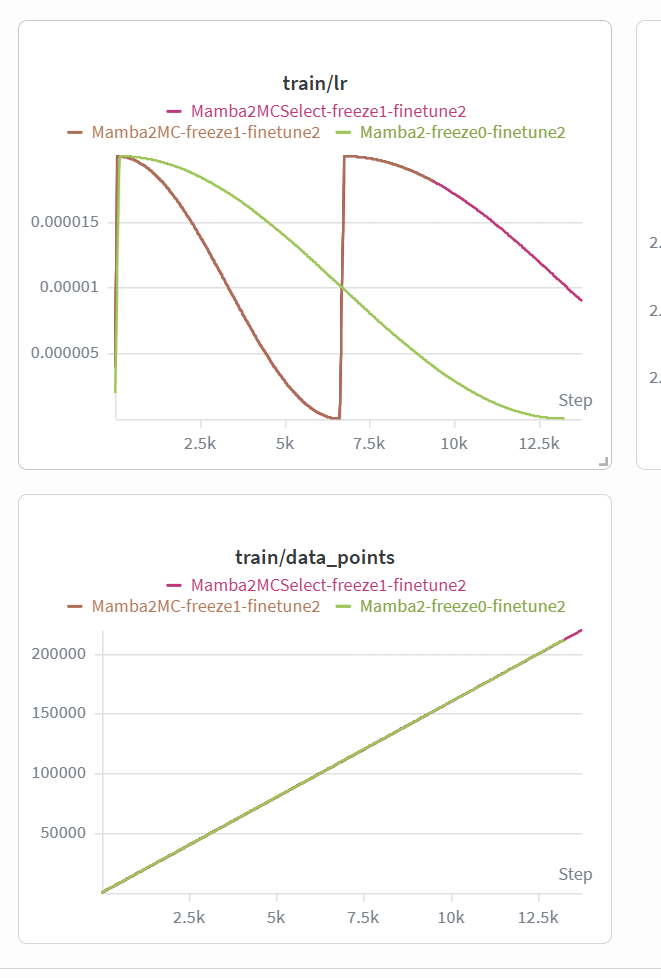
\includegraphics[width=0.95\linewidth]{figs/fig_lr.png}
\caption{Top: two-stage cosine learning-rate schedule---MC variants restart the cosine at the freeze$\to$finetune transition (step $\sim$6.5K), while the same-data baseline (green) runs a single cosine across 2 finetune epochs. Bottom: cumulative training data points (token packs) seen, identical across all three runs by construction.}
\label{fig:lr}
\end{figure}

\begin{figure}[t]
\centering
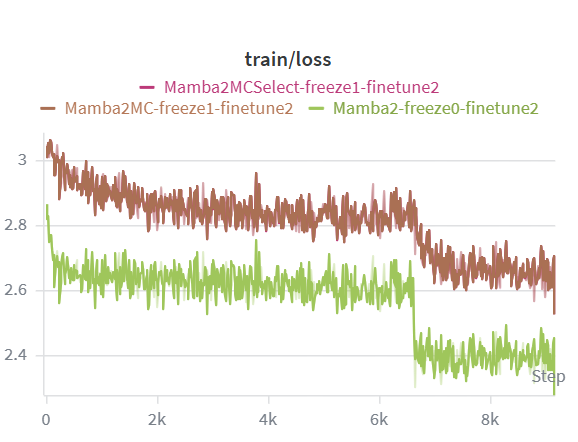
\includegraphics[width=0.95\linewidth]{figs/fig_loss.png}
\\\vspace{2pt}
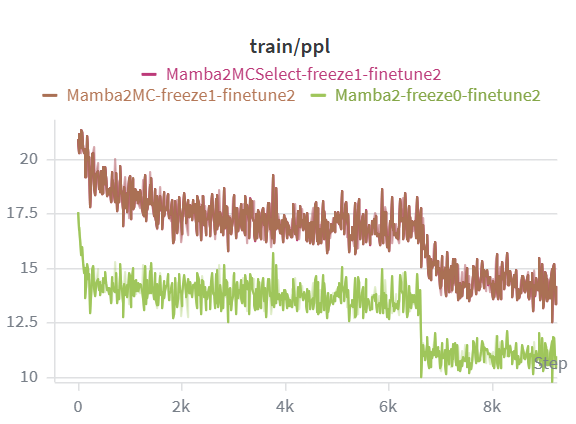
\includegraphics[width=0.95\linewidth]{figs/fig_ppl.png}
\caption{Training loss (top) and perplexity (bottom). The visible drop at $\sim$6.5K for MC corresponds to the freeze$\to$finetune transition.}
\label{fig:loss}
\end{figure}

\subsection{Discussion and Error Analysis}

\textbf{What works.} Both MC models reduce perplexity on the fine-tuning distribution, suggesting that $\beta$ may have opened and $W$ may have moved away from the identity into a meaningful query space (we did not log per-step parameter statistics, so this is inferred from the perplexity gap rather than measured directly). Mamba2MCSelect's $5$-point NIAH gain over Mamba2MC validates that selective retention beats FIFO eviction.

\textbf{What fails and why.} Five mechanisms compound. (1) \emph{Asymmetric training budgets}: $W$ alone has $d^2\!\approx 4.2$M parameters at $d{=}2048$; with $27$M tokens that is $\approx 6$ tokens per parameter, an order of magnitude below what an attention-style routing rule would need. (2) \emph{Mean-pooling is information-destructive}: $\bar h_k$ is a $64$-token mean---useful for coarse long-range retrieval (NIAH-like) but mostly noise for short-range fine reasoning (PIQA-style). (3) \emph{The gate is open}: $\sigma(\beta)\!\approx\!0.85$--$0.90$ at convergence, so $\approx 10$--$15\%$ of every prediction comes from the cache; combined with (1) and (2), this acts as a regulariser in the wrong direction on reasoning. (4) \emph{Detached cache} prevents the backbone from learning to produce better cache entries. (5) \emph{Distribution shift}: 2 epochs on WikiText+FineWeb narrows the broad calibration that PIQA/HellaSwag/ARC measure---this would happen with or without MC.

\textbf{Why MCSelect equals MC on reasoning.} With \texttt{block\_size}~$=256$ and segment size $64$, each training example contains at most $4$ segments---always below $K_{\max}{=}16$ and below $K{=}8$. The selection mechanism therefore \emph{never} actually evicts during training, and the scoring head receives essentially no gradient signal that would teach it to differentiate segments. The selector only kicks in at inference on long-context tasks (NIAH), which is exactly where the 5-point gap appears.

\textbf{Failure-mode analysis.} Combining mechanism (2) above with $\sigma(\beta)\!\approx\!0.85$--$0.90$ yields a concrete prediction: on short-context reasoning, the cache should add a small ($\sim$10--15\%) mostly-uniform perturbation to logits rather than a directed corruption, so MC and the baseline should fail on \emph{the same} items rather than on systematically different ones. A complete item-level failure overlap study was beyond the scope of this report but is a clean follow-up. On NIAH the prediction is the opposite---the cache should help precisely at depths where the recurrent state has begun to forget---which is consistent with the $0.85\!\to\!0.90$ improvement from MC to MCSelect.

%=============================================================
\section{Process}
\label{sec:process}
%=============================================================

\textbf{Pivot from the original proposal.} Our original proposal targeted three Mamba-2 efficiency upgrades (parallel inter-chunk associative scan, Triton-fused SSD kernels, and sequence parallelism) and a multi-turn dialogue memory benchmark. After the first weeks we re-scoped: the kernel and parallelism work would have produced engineering speedups but no new ML insight, and the dialogue benchmark we sketched overlapped substantially with NIAH-style retrieval, which already has a standardised evaluation. We pivoted to a single ML question---\emph{can a learnable cache fix the SSM recall gap?}---which directly motivated Mamba2MC and Mamba2MCSelect.

\textbf{Initialisation experiments that failed.} Early runs with $\beta=0$ (equal blending of $h_t$ and the cache mix) and a randomly-initialised $W$ produced loss spikes early in Stage 1 that did not recover within the budget. Switching to $\beta=8.0$, $W=I$, and a zero-init scoring head---making the model exactly behave like base Mamba-2 at step 0---was the single most important implementation decision and produced the stable curves in Figure~\ref{fig:loss}.

\textbf{Block-size discovery (mid-project).} Mid-project debugging revealed that with \texttt{block\_size}=256 each training sample contains only $4$ segments, far below $K_{\max}{=}16$ and below $K{=}8$, so MCSelect's TopK pruning never triggered during training. We did not have time to relaunch a larger-context run, but this finding is now the primary explanation for MCSelect's failure to differentiate from MC on the reasoning benchmarks.

\textbf{Engineering: dual forward paths and metadata.} A non-trivial engineering effort was making the segment-cache update both correct under sequential incremental inference \emph{and} fast under parallel chunk-aligned training. Our solution exposes all tokens within a single chunk to the same buffer snapshot in the fast path, which preserves Mamba-2's parallel throughput while keeping a strict step-by-step reference implementation for inference. We also wrote a checkpoint-metadata module to serialise cache hyperparameters with weights, after an early debugging incident where a mismatched $S$ silently degraded NIAH scores.

\textbf{Pending ablations.} Three follow-up experiments did not fit the project budget but would directly validate or revise our claims:
\emph{(A) Larger training context} (\texttt{block\_size}$\in\{1024,2048\}$): expected to produce the first non-trivial MCSelect-vs-MC gap on reasoning benchmarks by actually exercising the selector.
\emph{(B) Joint cache training} (\texttt{detach\_cached\_segments=False}): allows gradients to flow back through the cache, letting the backbone learn to produce better cache entries.
\emph{(C) Scaled data run} ($\ge 5$B tokens, diverse long-context corpus): the single most impactful next step. Each costs roughly $1$--$1.5$ GPU-days on our setup; together they would let us decompose the current ``MC underperforms'' result into its underlying causes.

\textbf{Lessons that generalise.}
\emph{(i) Initialisations matter more than architecture for fine-tuning stability}---always design new modules to have zero net effect at step 0.
\emph{(ii) Training geometry determines what the model can learn}---a cache-eviction or selection mechanism that never triggers during training cannot be expected to learn.
\emph{(iii) Architectural complexity has a data tax}---MCSelect is strictly more expressive than MC, but within $27$M tokens that extra expressivity bought us only the NIAH gain and nothing on reasoning.

%=============================================================
\section{Future Work}
%=============================================================

Beyond the three pending ablations above, longer-horizon directions include:
\begin{itemize}
    \item \emph{Adaptive segment boundaries}: replace fixed-size segments with learned splits at sentence or topic shifts.
    \item \emph{Jamba-style hybrid}~\cite{lieber2024jambahybridtransformermambalanguage}: interleave a few attention layers with MC-augmented SSM layers, getting Transformer-grade local recall without full $O(T^2)$ cost.
    \item \emph{Larger SSD state sizes}: the SSD framework supports much larger states than Mamba-1, which may reduce dependence on the explicit cache.
\end{itemize}

%=============================================================
\section{Conclusion}
%=============================================================

We proposed and implemented two memory-augmented extensions of Mamba-2: Mamba2MC, which maintains a sliding-window segment cache, and Mamba2MCSelect, which selectively retains high-scoring segments and uses them to bias attention. Trained on a $\sim$27M-token mix under a staged freeze-then-finetune protocol, both reduce in-distribution perplexity, and the selective variant improves long-context retrieval over the sliding-window variant. The fundamental bottleneck is data and training geometry: a $256$-token training context never exercises the cache eviction or the selector, so MCSelect's scoring head cannot receive useful gradient signal. The project's contribution is a reproducible proof-of-concept implementation and an analysis identifying both the promise and the prerequisites for memory-augmented SSMs.

%=============================================================
\section{Contributions}
%=============================================================

\begin{itemize}
    \item \textbf{Jinglu Sun.} Wrote the initial report draft and preliminary analysis. Coordinated the team schedule and coded the initial Mamba-2 model architecture used as the foundation for our later memory-augmented extensions.
    \item \textbf{Mo Jiang.} Designed the Mamba2MCSelect architecture, including the selective segment retention mechanism and score-biased attention. Developed the fine-tuning scripts, gathered the 27M-token training dataset, and managed the CARC SLURM cloud computing cluster job scripts for training support.
    \item \textbf{Zhenglong Liu.} Implemented the Mamba2MC sliding-window segment cache and developed sanity scripts for fine-tuning tests. Conducted the Needle-In-A-Haystack (NIAH) long-context retrieval benchmarking and performance evaluation.
    \item \textbf{Zhiyuan Jin.} Provided core idea guidance, such as dataset and benchmarking choice, for the memory-augmented SSM approach. Designed and ran the dataset-validation tests (token-count auditing, train/eval split sanity checks, and benchmark--training-set contamination checks for the WikiText+FineWeb mix). Performed the WikiText perplexity, PIQA, ARC, and HellaSwag benchmarking. Maintained the project GitHub repository and documentation, and led the final report revision and failure analysis.
\end{itemize}

%=============================================================
\section{AI Usage}
%=============================================================

We used Claude (Anthropic) to assist with: drafting and proofreading sections of this report; reviewing the cache-update and TopK-pruning logic; suggesting failure modes to look for in error analysis; and scouting candidate citations. Every cited paper was verified manually for existence and content. All architectural decisions, the implementation, the experiments, the training runs, and the final results are our own. The four authors reviewed the report end-to-end before submission and take full responsibility for its contents.

\bibliographystyle{ieeetr}
\bibliography{references}

\appendices

\section{Code}

The complete project code, including the Mamba-2 backbone, the Mamba2MC and Mamba2MCSelect modules, the fine-tuning driver, and the evaluation harness, is hosted at:

\url{https://github.com/Ruuuuuush2027/mamba2-optimization}

The repository's \texttt{README.md} lists the exact commands required to reproduce every result in this report (training, NIAH evaluation, and the WikiText / PIQA / HellaSwag / ARC benchmarks).

\section{Datasets}

All datasets are pre-existing public corpora; we did not collect or release a new dataset. We used:

\begin{itemize}
    \item \textbf{WikiText} ($\sim$10M training tokens). HuggingFace dataset card: \url{https://huggingface.co/datasets/wikitext}
    \item \textbf{FineWeb}, subset \texttt{CC-MAIN-2024-10} ($\sim$17M training tokens, streamed). HuggingFace dataset card: \url{https://huggingface.co/datasets/HuggingFaceFW/fineweb}
    \item \textbf{PIQA} (zero-shot evaluation). HuggingFace: \url{https://huggingface.co/datasets/piqa}
    \item \textbf{HellaSwag} (zero-shot evaluation). HuggingFace: \url{https://huggingface.co/datasets/Rowan/hellaswag}
    \item \textbf{ARC} (AI2 Reasoning Challenge, easy + challenge). HuggingFace: \url{https://huggingface.co/datasets/allenai/ai2_arc}
    \item \textbf{NIAH} (Needle-In-A-Haystack). Generated synthetically at evaluation time by our own re-implementation in \texttt{run\_benchmark.py}; the haystack text and needle templates are defined inline in the script.
\end{itemize}

The pre-trained Mamba-2 1.3B backbone is the official release from \texttt{state-spaces/mamba2-1.3b} (\url{https://huggingface.co/state-spaces/mamba2-1.3b}).

\section{Acknowledgements}

We build on the minimal PyTorch Mamba-2 implementation by \textit{tommyip} (\url{https://github.com/tommyip/mamba2-minimal}) and the official \texttt{state-spaces/mamba2-1.3b} pre-trained checkpoint. Training uses HuggingFace \texttt{transformers} and \texttt{datasets}; zero-shot reasoning is evaluated with the \texttt{lm-evaluation-harness}. The NIAH evaluation is a self-contained re-implementation. All starter code is credited inline in the repository.

\end{document}
